\documentclass{pnastwo}
\usepackage{color}
\usepackage{graphicx}
\usepackage{amssymb,amsfonts,amsmath}
\usepackage{lineno}
\usepackage{multirow}
\usepackage{color}
	 \definecolor{darkred}{rgb}{0.75,0,0}
	 \definecolor{darkgreen}{rgb}{0,0.5,0}
	 \definecolor{darkblue}{rgb}{0,0,0.75}
\newcommand{\cha}[1]{\textcolor{darkblue}{#1}}
\newcommand{\arne}[1]{\textcolor{darkred}{#1}}


\usepackage[sort&compress]{}


\begin{document}

\title{Population dynamics of mutualisms}

 \author{Chaitanya S. Gokhale\affil{1}{New Zealand Institute for Advanced Study, Massey University, Auckland, New Zealand}}


\maketitle

\begin{article}

\begin{abstract}
Mutualistic relationships pose a conundrum for evolutionary theory.
Species that exploit other species would do better than sustaining a long drawn out mutually costly relationship. However we do see mutualistic relationships amongst even the most unlikely partners \ldots.
Eco-evolutionary dynamics \ldots
\end{abstract}


\keywords{mutualism | evolutionary game theory | multiple players
}

\section{Introduction}

In his book 'The History of Animals', Aristotle observes
{\em
`When the crocodile yawns, the trochilus flies into his mouth and cleans
his teeth. The trochilus gets his food thereby, and the crocodile
gets ease and comfort; it makes no attempt to injure its little friend,
but, when it wants it to go, it shakes its neck in warning, lest it
should accidentally bite the bird'} \cite{aristotle:350bc}.
The phenomenon described by Aristotle was termed as mutualism in $1873$ by the Belgian zoologist Pierre van Beneden \cite{bronstein:book:2003}.
Mutualistic relationships, interspecific interactions that benefit both species, have been empirically studied for many years 
\cite{boucher:book:1985,hinton:PTENHS:1951,wilson:AmNat:1983,bronstein:QRB:1994,pierce:ARE:2002,kiers:Nature:2003,bshary:ASB:2004} and also a considerable body of theory has been put forth trying to explain the evolution and maintenance of such relationships \cite{poulin:JTB:1995,doebeli:PNAS:1998,noe:book:2001,johnstone:ECL:2002,bergstrom:PNAS:2003,hoeksema:AmNat:2003,akcay:PRSB:2007,bshary:Nature:2008}.
The example described by Aristotle and most other examples of mutualisms lend themselves to the idea of direct reciprocity \cite{trivers:QRB:1971} and thus can be studied using evolutionary game theory.
The interactions in these models are usually dyadic.
A representative of each species is chosen and the outcome of the interactions between these representatives 
determines the evolutionary dynamics within each of the two species.
However, in many cases interactions between species cannot be reduced to such dyadic encounters \cite{stadler:book:2008}.

For example, in the interaction between ants and aphids or butterfly larvae \cite{pierce:BES:1987,hoelldobler:book:1990} many ants tend to these soft bodies creatures, providing them with shelter and protection from predation and parasites in exchange for honeydew, a rich source of food for the ants \cite{hill:OEC:1989,stadler:book:2008}.
This is not a one to one interaction between a larva and an ant, but rather a one to many interaction from the perspective of the larva.
In this manuscript we focus on this kind of -- possibly -- many to many interactions between two mutualistic species.

To analyze how benefits are shared between the two mutualistic species, we make use of evolutionary game theory.
Since we consider the interaction of two species, we resort to bimatrix games
\cite{weibull:book:1995,hofbauer:JMB:1996,hofbauer:book:1998}.



\section{Model and Results}

\subsection{Interspecies dynamics}

\subsection{Intraspecies dynamics}

Usually when interspecies relationships such as mutualism (or antagonist relationships as in predator-prey) are considered, the within species interactions are ignored for the sake of convenience. Including intraspecies interactions can however result in qualitatively different and rich dynamics which has implications for interspecies relationships.
Since we focus on mutualism the interspecies dynamics  ifs given by the multiplayer version of the snowdrift game \cite{bergstrom:PNAS:2003,souza:JTB:2009,gokhale:PRSB:2012}.
Each species consists of two types of individuals Generous $G$ and Selfish $S$. 
The details of the game are included in the Appendix, but the gist is that if everyone is Generous and contributing in the generation of mutual benefits then one can get away with being a bit selfish. All selfish is however and unstable equilibrium 

\subsection{Combined dynamics}

\subsection{Population dynamics}
%Consider two species ($1/2$) occupying different niches in an ecosystem.
%Thus we assume them to have independent carrying capacities. Each species has a normalized carrying capacity of $1$. Each species has two types the \textit{``Generous"} ones ($G_{1/2}$) who invest in a mutualistic relationship with the other species and \textit{``Selfish"} ones ($S_{1/2}$) who invest much less than their counterparts. The densities of the two types are denoted by $x_{1/2}$ and $y_{1/2}$ respectively which can sum up to the carrying capacity or not thus resulting in possible empty spaces in the niche $z_{1,2}$. Thus in all we have $x_{1/2} + y_{1/2} + z_{1/2} = 1$.
%Thus how the population densities change over time $x_{1/2} + y(1/2)$ can give us a picture of the population dynamics.
%\subsection{Evolutionary dynamics}
%The two species are assumed to be engaged in a mutualistic relationship. This can be aptly described by a snowdrift game \cite{souza:JTB:2009}. In a general form, a number of individuals from one species interacts with a number of individuals from the other species (excluding intra species interactions) \cite{gokhale:PRSB:2012}. 
%The densities of the two types of individuals in each species \textit{``Generous"} and \textit{``Selfish"} can be interpreted as probabilities of picking the two types. Thus the evolution of the fraction of one of the types, say \textit{``Generous"} over time provides us with the relevant evolutionary dynamics. The fraction of \textit{``Generous"} players is given by $f_{1/2} = x_{1/2} / (1- z_{1/2} )$.

\begin{figure}[h]
\begin{center}
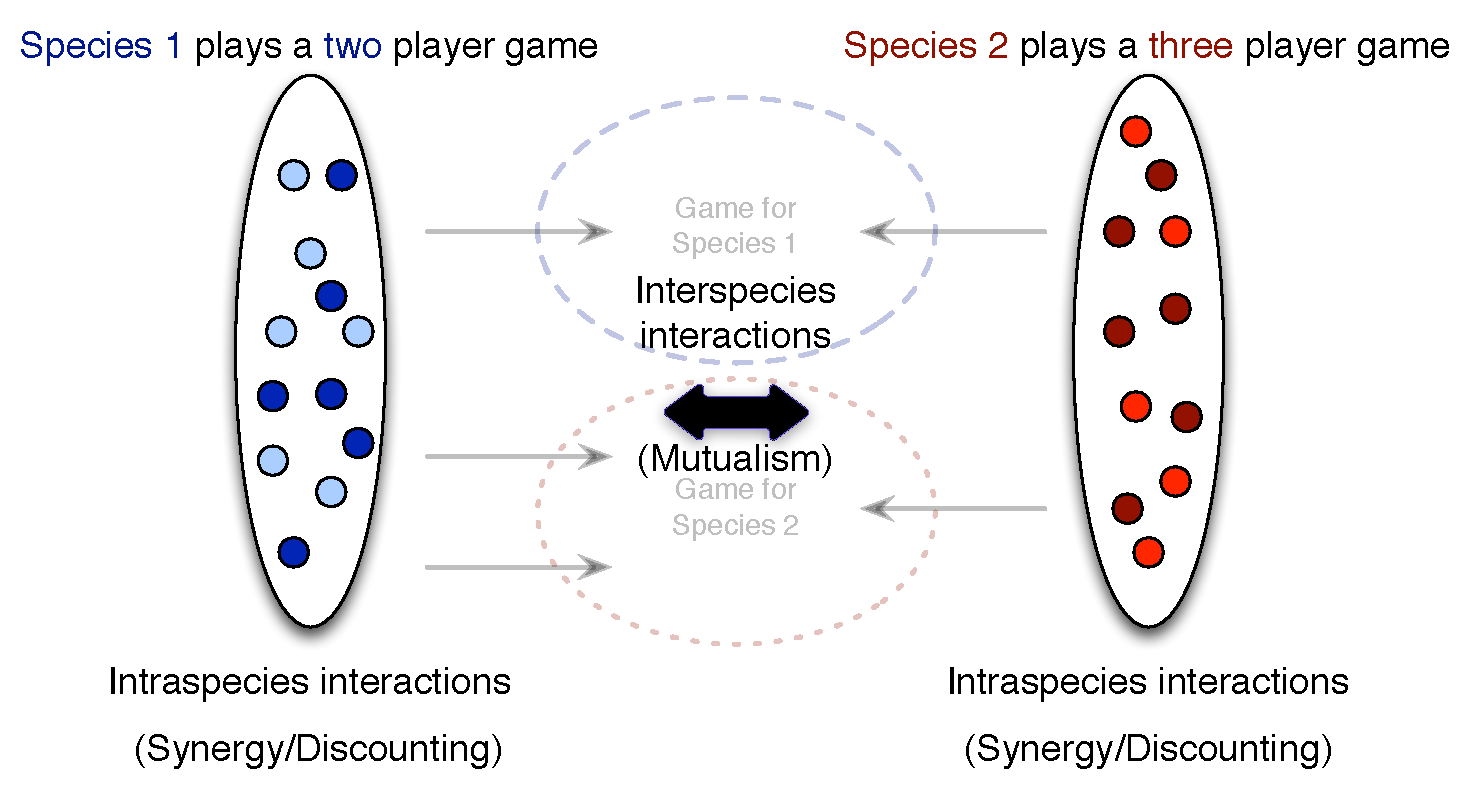
\includegraphics[width=\columnwidth]{../Figures/interintra.pdf}
\caption{
Explain figure
}
\end{center}
\end{figure}

\section{Discussion}




\begin{acknowledgments}
Thanks for all the fish
\end{acknowledgments}




\appendix

\section*{Appendix}

\section*{Average payoffs from interactions between species}
\label{appA}

The two species are assumed to be in a mutualistic relationship.
Following \cite{bergstrom:PNAS:2003,souza:JTB:2009,gokhale:PRSB:2012}, we make use of the multi-player version of the snowdrift game to represent a co-existence scenario.
Each species has two types of individuals ``Generous" ($G$) and ``Selfish" ($S$).
Say the frequency of $G$ individuals in species $1$ is given by $x$ and that in species 2 by $y$
Each individual from each species takes part in a $d$ player interspecies game where it interacts with $d-1$ individuals from the other species.
Of the $d-1$ the if $k$ of them are $G$ while $d-1-k$ are $S$ then the payoff accrued by the individuals is given by,
%
\begin{align}
f^{inter}_{G_1} (y) &= \sum_{k=0}^{d-1} \binom{d-1}{k}y^k (1-y)^{d-1-k} \Pi_{G_1}(k+1) \\
f^{inter}_{S_1} (y) &= \sum_{k=0}^{d-1} \binom{d-1}{k}y^k (1-y)^{d-1-k} \Pi_{S_1}(k).
\label{interfiteqs}
\end{align}
%
for the two types in species 1.
Analogously the fitness for the two types in species 2 can be written down as $f^{inter}_{G_2} (x)$ and $f^{inter}_{S_2} (x)$ which depend on the frequencies of $G$ in species 1.
The payoff for a $G$ thus includes itself ($k+1$) while for a $S$ individual only the the number of $G$ matter ($k$).
The payoffs themselves are defined as in \cite{souza:JTB:2009},
%
\begin{align}
\Pi_{S_1} (k) & = \begin{cases} b & \textrm{if } k \geq M \\ 0 & \textrm{if } k < M \end{cases}
\\
\Pi_{G_1} (k) & = \begin{cases} b-\frac{c}{k} & \textrm{if } k \geq M \\  -\frac{c}{M} & \textrm{if } k < M \end{cases}
\end{align}
%
The selfish players get the benefit $b$ if the number of generous individuals in the interacting group, $k$, is greater than or equal to the threshold $M$.
For the generous individuals, their effort is subtracted from the payoffs.
The effort is shared if the quorum size is met ($\frac{c}{k}$), but is in vain for $k<M$.


\section*{Average payoffs from interactions within species}
\label{appB}

Within a species we do not assume a certain kind of interaction structure.
Instead we model the interaction matrix by making use of a general framework of costs and non-linear benefits \cite{eshel:AmNat:1988,hauert:JTB:2006a} which can potentially encompass all different types of social interaction structures qualitatively.
A crucial \textbf{assumption} which we make here is that the ``Generous" individuals from the between species interactions are the ``Cooperative" ones in the within species interaction and the ``Selfish" ones are the ``Defectors".
Hence for species 1 the frequency of cooperators is just $x$ and the defectors is $1-x$, the same as the ``Generous" and ``Selfish".
Again for simplicity we \textbf{assume} a $d$ player game being played within species, the same as in between species.
Thus the fitnesses of cooperators and defectors are defined as \cite{hauert:JTB:2006a},
%
\begin{align}
	f^{intra}_{G_1} (x) &= \sum_{k=0}^{d-1} \binom{d-1}{k}x^k (1-x)^{d-1-k} \Gamma_{G_1}(k+1) \\
	f^{intra}_{S_1} (x) &= \sum_{k=0}^{d-1} \binom{d-1}{k}x^k (1-x)^{d-1-k} \Gamma_{S_1}(k).
\label{intrafiteqs}
\end{align}
%
where the payoffs are given by,
\begin{align}
	\Gamma_{S_1} (k) = \frac{\tilde{b}}{d} \sum_{i=0}^{k-1} \omega^i \\
	\Gamma_{G_1} (k) = \Gamma_{S_1} (k) - \tilde{c}.
\end{align}
%
Thus the defectors get a fraction of the benefit which is scaled by the factor $\omega$, which determines if the benefits are linearly accumulating ($\omega=1$) for increasing number of cooperators, synergistically enhanced ($\omega>1$) or saturating ($\omega<1$).
Note that the costs and benefits in the within species game need not be (and naturally so) the same as in between species ($b\neq \tilde{b}$ and $c \neq \tilde{c}$).


\section{Average payoffs and dynamics}

The average payoffs are then just assumed to be a linear combination of the interspecies and intraspecies interactions where the parameter $p$ determines the strength of each of the interactions such that,
%
\begin{align}
	f_{G_1} (x,y) &= p f^{inter}_{G_1} (y) + (1-p) f^{intra}_{G_1} (x) \\
	f_{S_1} (x,y) &= p f^{inter}_{S_1} (y) + (1-p) f^{intra}_{S_1} (x)
\label{fiteqs}
\end{align}
%
Following the same procedure for the two strategies in species $2$ leads to the average fitness
%
\begin{align}
\bar{f}_1 (x,y) &= x f_{G_1} (y)+(1-x) f_ {S_1}(y)\\
\bar{f}_2 (x,y) &= y f_{G_2} (x)+(1-y) f_{S_2}(x).
\label{avgfiteqs}
\end{align}
%
The time evolution of the ``Generous" types in all the species will give us the complete dynamics of the system.
However since the two interaction species are by definition different organisms, they can have different rates of evolution.
Thus if species 1 evolves at the rate $r_x$ while species 2 at rate $r_y$ then we have,
\begin{align}
\dot{x} &= r_x x \left(f_{G_1}(y) -  \bar{f}_1(x,y) \right) \nonumber \\
\dot{y} &= r_y y \left(f_{G_2}(x) -  \bar{f}_2(x,y) \right).
\label{eq:repeqs}
\end{align}



\cha{\section{Asymmetries}}

\cha{This between and within species model is a powerful way of introducing a lot of variability into the dynamics,
\begin{align}
	d_1 &\neq d_2 \\
	d^{inter} &\neq d^{intra} \\
	M_1 &\neq M_2 \\
	b &\neq \tilde{b} \\
	c &\neq \tilde{c} \\
	r_x &\neq r_y \\
	&\vdots
\end{align}
and various combinations of these. We should justify why we don't do this here and why we do vary the ones that we do.}


\section{Dynamics in asymmetric conditions}

%We have addressed two kinds of asymmetries in the game, the number of player and the thresholds in the two species.
%We denote the number of players for species $1$ and species $2$ as $d_1$ and $d_2$, respectively, as in Fig.\ \ref{fig:counter}.
%That is if species $2$ is playing a $d_2$ player game it means that one player from species $2$ interacts with $d_2-1$ players of species $1$.
%For an asymmetry in the thresholds we use the two parameters $M_1\geq1$ and $M_2\geq1$ for the two species, respectively.

For asymmetric bimatrix games, there is a difference in the dynamics between the standard replicator dynamics and the 
alternative dynamics put forward by Maynard-Smith \cite{maynard-smith:1982to}.
For this dynamics, the average fitness of each species appears as a denominator,
\begin{align}
\dot{x} &= r_x x \left(f_{G_1}(y) -  \bar{f}_1(x,y) \right)/\bar{f}_1(x,y) \nonumber \\
\dot{y} &= r_y y \left(f_{G_2}(x) -  \bar{f}_2(x,y) \right)/\bar{f}_2(x,y).
\label{eq:repeqs}
\end{align}
In our asymmetric bimatrix game, the fixed point stability is affected by the choice of the dynamics, in contrast to the case of symmetric games. 
In Fig.\ \ref{fig:thresholdsmodrep}, we illustrate that the dynamics is different between the usual 
replicator dynamics and Eqs. \ref{eq:repeqs}

For $d_1=d_2 \geq 5$, the exact coordinates of the fixed point must be computed numerically \cite{abel:1824aa,stewart:2004aa}.

\bibliographystyle{pnas}
\bibliography{\string~/Bibtex/et.bib}


\end{article}
\end{document}